\graphicspath{{chapters/08/images8/}}
\chapter{Genome wide association studies}

\section{Observational studies}
\textbf{Observational} studies can be divided in two categories: \textbf{descriptive} and analytical.
The main idea is to observe a sample of population and extract information about environmental and/or genetic characteristics wrt specific genetic or phenotype marks (often, diseases).

	\subsection{Descriptive studies}
	Descriptive studies are studies in which an \textbf{hypothesis} is generated.
	Then the patterns of disease occurrence in relation to variables such as person, place and time are studied.
	They are often the first step or initial inquiry into a new topic event, disease or condition.
	They typically estimate the frequency and the magnitude of the event analyzed.

	\subsection{Analytical studies}
	Analytical studies take the descriptive studies a step forward.
	An analytical study is one in which action will be taken on a cause system to improve the future performance of the system of interest.
	The focus is to test an hypothesis to produce predictive data.
	In particular they are used to identify factors that are associated with a disease or to quantify the risk of these factors.
\\
Analytical studies can be ulteriorly divided into cohort and case studies.
	
	\subsubsection{Cohort studies}
	\textbf{Cohort} studies are a type of analytical studies that involve a cohort.
	\textit{A cohort is a well-defined group of individuals who share a common characteristic or experience}.
	For example individual exposed to a drug, vaccine or pollutant.

		\paragraph*{Prospective cohort studies}
		Prospective cohort studies potential exposure has already occurred while outcomes have yet to occur.
		Participants are grouped according to past or current exposure and a follow-up in the future determine whether the predicted outcome occurs.

		\paragraph*{Retrospective cohort studies}
		Retrospective cohort studies both exposure and outcomes have already occurred.
		Participants are grouped according to past exposure and certain characteristics and are compared for a particular outcome.
		
		\begin{figure}[H]
		\centering
		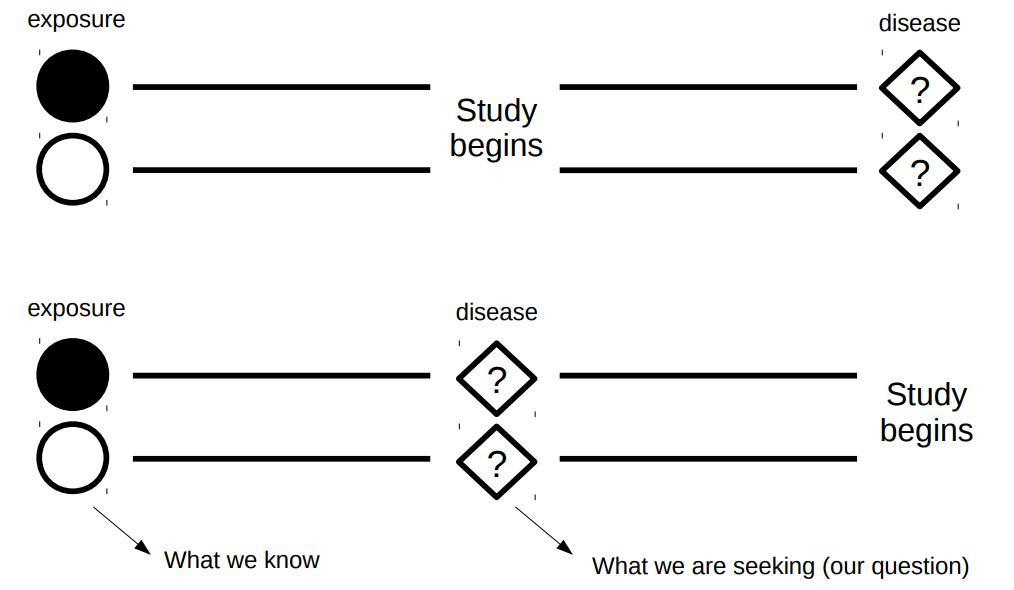
\includegraphics[scale=0.2]{cohort}
		\caption{Prospective and retrospective cohort studies.}
		\end{figure}

		\subsubsection{Measures of associations}
		In cohort study a $2\times 2$ table can be built to determine, for example, the effect of exposure to a certain event on disease presence.
		This type of table is described on table \ref{tab:risk_table}.

		\begin{table}[H]
			\centering
			\begin{tabular}{ccc}
				 & \multicolumn{2}{c}{Disease}\\
				 & Yes & No \\
				 \cline{2-3}
				 Exposed & \multicolumn{1}{|c|}{$a$} & \multicolumn{1}{|c|}{$b$}\\
				 \cline{2-3}
				 Not exposed & \multicolumn{1}{|c|}{$c$} & \multicolumn{1}{|c|}{$d$}\\
				 \cline{2-3}
			\end{tabular}
			\caption{Cohort study's table example}
			\label{tab:risk_table}
		\end{table}
		
		From such a table we can define three main measures of association:
		
		
		\begin{description}
		\item[Strength of association: Relative Risk (RR) and Risk Excess (RE)]
			
			First, from this table the percentage of individuals exposed harboring the disease can be computed:

		$$I_e = \frac{a}{a+b}$$

		Also the percentage of individuals not exposed and not harboring the disease:

		$$I_{ne} = \frac{c}{c+d}$$

		From this two measure the risk excess $RE$ and the relative risk $RR$ can be computed:

		$$RE = I_e - I_{ne} \qquad\qquad RR= \frac{I_e}{I_{ne}}$$

		The risk excess determine how the exposure betters, or worsen the chance of presenting a disease.
		The relative risk instead determine the nature of the exposure's event:

			\begin{itemize}
				\item $RR<1$ indicates a protective factor: incidence of developing the disease is much lower when the population is exposed to an event.
				\item $RR \sim 1$ indicates an absence of risk.
				\item $RR> 1$ indicates a risk factor.
			\end{itemize}
	
		
		\item[Precision of association: Confidence Interval (CI)]
		Remember, the risk is calculated always in a sample of the population.
		It is a range of values, on the basis of the sample data, in which the population value (or true value) may lie.
		\\
		Formal definition of CI: \textit{If the measurement of the estimate could be replicated many times, the correct value is inside the interval $95\%$ (or $90\%$ or $80\%$...) of the time.}
		In practice, we can be reasonably confident that the correct value (which is the one we are observing in a population) is inside the confidence interval.
		\\
		Usually the relative risk indicates the amount of random error around the point estimate.
		The formula for calculating the $RR$ the becomes something like:
			$$RR = point estimate \,(lower confidence limit - upper confidence limit)$$
			Where the subtraction in the parenthesis represent the confidence interval.
			
		\item[Significance of association: p-value (P)]
		From the table also a significance of association can be computed.
			It requires a $p$-value, that determine how unlikely it is that the events observed arise by chance.
		
		\end{description}
			

	\subsection{Case-control study}
	The purpose of a case-control study is typically to study rare diseases or multiple exposures (or genetic factors) that may be related to a single outcome.
	Participants are selected based on \textbf{outcome} status and therefore divided in two categories, case- and control-subjects:

	\begin{multicols}{2}
		\begin{itemize}
			\item Case subjects have outcome of interest.
			\item Control subjects do not have outcome of interest.
		\end{itemize}
	\end{multicols}

	This type of study is usually preferred when funding is limited.

		\subsubsection{Measure of association}
		The same table as a cohort study is built (as in table \ref{tab:risk_table}), but the measure of strength of association is different.
		
		\begin{description}
		\item[Strength of association: Odds Ratio (OR)]
		First the odds\footnote{An odd is a ratio of probabilities, ratio between the probability that an event will happen and the probability that an event will not happen.} of exposure in cases is computed:

		$$\frac{\frac{a}{a+c}}{\frac{c}{a+c}} = \frac{a}{c}$$

		Then the odds of exposure in control:

		$$\frac{\frac{b}{b+d}}{\frac{d}{d+b}} = \frac{b}{d}$$

		Finally the ratio of this two measure is the odds ratio $OR$, the measure of association for a case control study:

		$$OR = \frac{\frac{a}{c}}{\frac{b}{d}} = \frac{ad}{bc}$$

		$OR$ is in relationship with $RR$ following the equation:

		$$OR = \frac{RR(1-R_0)}{1-RR\cdot R_0}$$

		Where $R_0$ is the frequency of the disease in the not exposed population.

		$OR$ can be interpreted like $RR$:

		\begin{multicols}{3}
			\begin{itemize}
				\item $OR <1$: protective factor.
				\item $OR = 1$: absence of risk.
				\item $OR > 1$: risk factor.
			\end{itemize}
		\end{multicols}
		
		\item[Significance of association: p-value (P)]
		\item[Precision of association: Confidence Interval (CI)]
		\end{description}
		
		\subsubsection*{Relation between RR and OR}
		$RR$ and $OR$ are two different measures, derived from two different types of studies, one searching for the exposure and one searching for the outcome.
		Some mathematical relation exists between these two measures, that tells us that when the disease is rare, mathematically the $RR = OR$. 
		A graphical representation of this relation is depicted in figure \ref{fig:divergence}.
		The difference is that the $RR$ is \textit{immediate}, meaning that if a person has probability $2$ of developing a disease, it is the same as saying that it has double the risk of developing it of a person not exposed. 
		With $OR$ instead, this reasoning is not immediate.
		
		\begin{figure}[H]
		\centering
		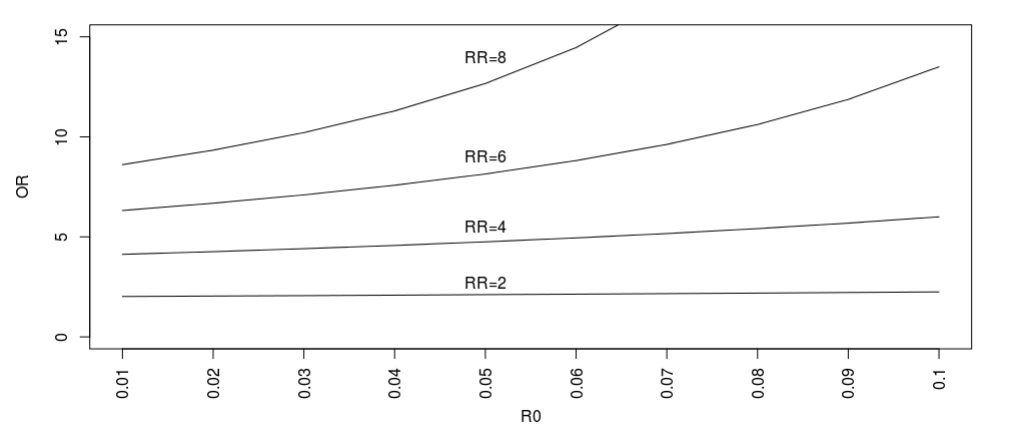
\includegraphics[scale=0.3]{divergence}
		\caption{The more a disease is rare, the stronger the correlation is. On the contrary, if the disease in a population is not that uncommon, we can see a divergence between OR and R0, where R0 is the frequency of the disease in the not exposed population.}
		\label{fig:divergence}
		\end{figure}



\section{GWAS}
	\subsection{Objective of GWAS}
	The objective of a GWAS is to find connections between a phenotype (height, type-I diabetes, etc.,) known to be heritable and whole-genome genotype.
	GWAS were developed in $2004$, mainly thanks to the HapMap project, which unraveled the existence of linkage disequilibrium blocks, which allowed the exploitation of tag SNPs.
	Particularly important was the realization, after the discovery of the haplotype blocks, that not all of human genetic variation (millions of SNPs) had to be genotypes to find associate variants, but  only a fraction of those (\textbf{tag SNPs}).
	Specific goals are distinct:

		\begin{itemize}
			\item \textbf{Identification of statistical connections between points or areas in the genome and the phenotype.
				The hypotheses are driven for biological studies of specific genes or regions in specific contexts.}
			\item Generation of insights on genetic architecture or phenotype.
				In fact a phenotype could be due to many small genetic effects dispersed across the genome or due to few large effects concentrated in one area.
				An example in the second case is the MHC or major histocompatibility complex, a group of genes involved in the mechanism of immune defense.
			\item Build statistical models to predict phenotype from genotype.
		\end{itemize}


	\subsection{Main applications of GWAS}
	 An overview of the possibilities provided by GWAS are reported in figure \ref{fig:potential}.
	 \begin{figure}
	 \centering
	 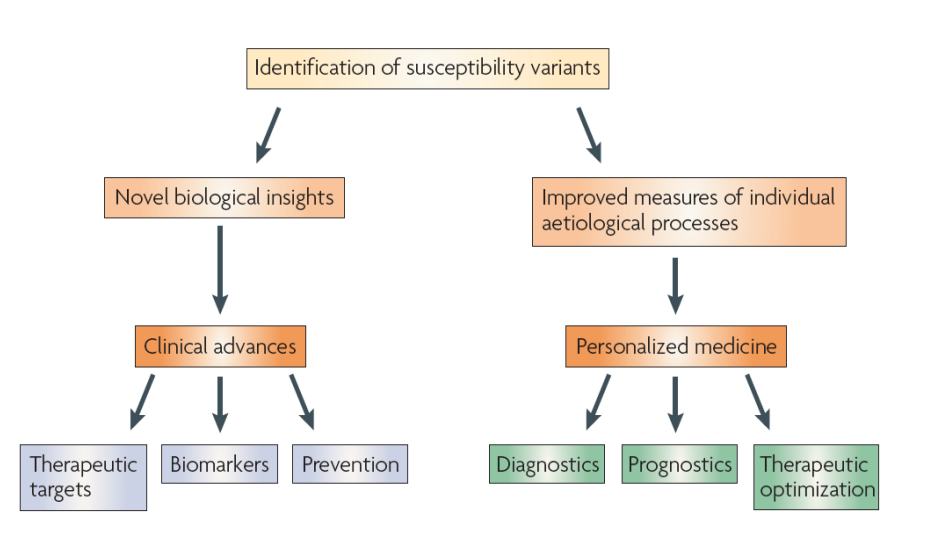
\includegraphics[scale=0.3]{potential}
	 \caption{Potential of GWAS and main possible applications}
	 \label{fig:potential}
	 \end{figure}
	 

	\subsection{GWAS methodology}
	A typical GWAS methodology can be described as:

		\begin{itemize}
			\item Collect $n$ subjects with known phenotype, usually $n\in [10^3;10^4]$.
			\item Measure each one in $m$ genomic locations representing common variation in the whole genome.
				Typically these are SNPs.
				Usually $m\in [10^5;10^6]$, but recently with whole genome sequencing $m = 3\cdot 10^9$.
			\item The data can be thought as a matrix $X$ of dimension $n \times m$ with subject as rows and SNPs as columns.
				This matrix is built such that $X_{ij} \in \{0,1,2\}$, representing the genotype at a single column.
				Moreover a vector of phenotypes $Y_n$ can be given.
		\end{itemize}

	Having collected the data and having computed the matrix $X$ and the vector $Y$ the first task is \textbf{association testing}: finding SNPs (column of $X$) that are statistically associated with $Y$.
	This can be thought of as $m$ separate statistical tests run on the matrix $X$.

	\subsection{Single nucleotide polymorphisms}
	In general, genetic polymorphisms are genetic variants that have a prevalce greater than 1\% in the population.
	There are different type of polymorphisms:
	\begin{itemize}
	 \item \textbf{Single Nucletoide Polymorphisms (SNPs)}, which will be our main focus;
	 \item Small-scale insertions and deletions;
	 \item Microsatellite variations;
	 \item Copy Number variations.
	 \end{itemize} 
	 
	A SNP is defined as a single base variation in a DNA sequence.
	They are classified according to the minor allele frequency $MAF$\footnote{Minor allele frequency (MAF) is the frequency at which the second most common allele occurs in a given population. They play a surprising role in heritability since MAF variants which occur only once, known as "singletons", drive an enormous amount of selection. (Wikipedia)}

	\begin{multicols}{2}
		\begin{itemize}
			\item Common SNPs have $MAF \ge 1\%$.
			\item Rare SNPs have $MAF < 1\%$.
		\end{itemize}
	\end{multicols}

		\subsubsection{SNPs frequency}
		In the human genome SNPs compose the $0.1\%$ and are what makes human unique.
		These variants can be:

		\begin{multicols}{3}
			\begin{itemize}
				\item Harmless, change only the phenotype;
				\item Harmful, associated with a multitude of diseases;
				\item Latent, can become detrimental only in particular conditions (genetic-environmental cooperation).
			\end{itemize}
		\end{multicols}

		They can lie in coding regions, but the majority of them are found in non-coding one.
		Thy are present between in $1$ every $1000$ bases or $1$ every $100$-$300$.
		The abundance of SNPs and the ease with which they can be measured make them very important.
		Two thirds of SNPs modification are from a $C$ to a $T$.
		They are typically found in non-coding regions and are found less in less conserved regions.
		In coding regions synonymous SNPs (that don't change the structure of the coded protein) are more common.

		\subsubsection{SNPs effects}
		SNPs can have different effect on the genome:

		\begin{multicols}{2}
			\begin{itemize}
				\item When they are found near a gene they can act as marker for that gene.
				\item SNPs in regulatory regions can modify transcription influencing the binding of transcription factors.
				\item SNPs in coding regions can modify the stricture of codified protein.
			\end{itemize}
		\end{multicols}

		\subsubsection{Nucleotide diversity}
		Nucleotide diversity measures the degree of polymorphism in DNA sequences or in a population.
		It is defined as the average number of nucleotide differences per site between two DNA sequences in all possible pairs in the same population and is denoted by $\pi$
		It is estimated as:

		$$\hat{\pi} = \frac{n}{n-1}\sum\limits_{ij} x_ix_j\pi_{ij} = \frac{n}{n-1} \sum\limits_{i=2}^n\sum\limits_{j=1}^{i=1}2x_ix_j\pi_{ij}$$

		Where:

		\begin{multicols}{2}
			\begin{itemize}
				\item $x_i$ and $x_j$ are the respective frequencies of the $ith$ and $jth$ sequences.
				\item	$\pi_{ij}$ is the number of nucleotide differences per nucleotide site between the $ith$ and $jth$ sequences.
				\item $n$ is the number of sequences in the sample.
				\item $\frac{n}{n-1}$ is a normalization factor that makes the estimator independent on how many sequences are sampled.
			\end{itemize}
		\end{multicols}

			\paragraph{Hardy-Weinberg equilibrium}
			In a population with genotypes $BB$, $bb$ and $Bb$, if:

			\begin{multicols}{2}
				\begin{itemize}
					\item $p = freq(B)$.
					\item $q = freq(b)$.
				\end{itemize}
			\end{multicols}

			The frequencies of the genotypes are then:

			\begin{multicols}{3}
				\begin{itemize}
					\item $freq(BB) = p^2$.
					\item $freq(bb) = q^2$.
					\item $freq(Bb) = 2pq$
				\end{itemize}
			\end{multicols}

			In a condition of equilibrium and will not change considering:

			\begin{multicols}{3}
				\begin{itemize}
					\item No mutations.
					\item No emigrations.
					\item Population of infinite size.
					\item No selective pressure.
					\item Random coupling.
				\end{itemize}
			\end{multicols}

		\subsubsection{Linkage disequilibrium}
		Two genetic loci are said to be in linkage disequilibrium $LD$ when there is a non-random association of alleles at different loci in a given population.
		It usually indicates that two alleles are near and in mammalians $LD$ is usually lost at around $100Kbp$.
		Let:

		\begin{multicols}{2}
			\begin{itemize}
				\item $p_A$ be the frequency of an allele $A$ in a genomic locus.
				\item $p_B$ be the frequency of an allele $B$ in another genomic locus.
			\end{itemize}
		\end{multicols}

		The association between allele $A$ and allele $B$ is random when:

		$$p_{AB} = p_Ap_B$$

			\paragraph{Measuring linkage disequilibrium}
			The coefficient $D$ is a measure of linkage disequilibrium.
			It is defined for two biallelic loci with alleles $A$ and $a$ at the first locus and $B$ and $b$ at the second one as:

			$$D_{AB} = p_{AB} - p_Ap_B\qquad\qquad D_{Ab} = -D_{AB}\qquad\qquad D_{ab} = D_{AB}$$

			Being $LD$ a property of two loci and not of their alleles, it is the magnitude being of interest, not the sign.
			The magnitude does not depend on the choice of the allele, and the range of $D$ changes with allele frequency.
			Knowing that $p_{AB}$ is smaller than $p_A$ and $p_B$ and that the frequencies cannot be negative:

			$$-p_Ap_B\land -p_ap_b\le D_{AB}\le p_ap_B\land p_Ap_b$$

			The possible values of $D$ depend on the allele frequencies and as such is difficult to interpret.
			Because of this it is normalized in $D'$:

			$$D'_{AB} = \begin{cases}\frac{D_{AB}}{\max(-p_Ap_B, -p_ap_b)} & D_{AB} < 0\\\frac{D_{AB}}{\min(p_ap_B, p_ap_b)} & D_{AB}>0\end{cases}$$

				\subparagraph{Measuring LD with $r^2$}
				To measure $LD$ with $r^2$ two random variables are defined:

				\begin{multicols}{2}
					\begin{itemize}
						\item $X_A$ such that $X_A=1$ if allele at locus $1$ is $A$ and $X_A=0$ if the allele is $a$.
						\item $X_B$ such that $X_B=1$ if allele at locus $2$ is $B$ and $X_B=0$ if the allele is $b$.
					\end{itemize}
				\end{multicols}

				Or:

				$$X_A = \begin{cases}1 & allele=A\\0 & allele = a\end{cases}\qquad\qquad X_B = \begin{cases}1 & allele = B\\0 & allele = b\end{cases}$$

				Then the correlation between the two random variables can be defined as:

				$$r_{AB} = \frac{Cov(X_A, X_B)}{\sqrt{Var(X_A)Var(X_B)}} = \frac{D_{AB}}{\sqrt{p_A(1-p_A)p_B(1-p_B)}}$$

				And:

				$$r^2_{AB} = \frac{D^2_{AB}}{p_A(1-p_A)p_B(1-p_B)}$$

				This measure is usually employed as it is always a positive value.

				\subparagraph{Classifying LD}
				$LD$ can be classified according to the $D'$ and $r^2$ values:

				\begin{multicols}{2}
					\begin{itemize}
						\item When $D'= 1$ there is complete $LD$.
						\item When $r^2 = 1$ there is perfect $LD$.
					\end{itemize}
				\end{multicols}

				Perfect $LD$ implies complete $LD$.
				There are situations in which $D'=1$ and $r^2$ is low, so usually both measures are reported.
				
				\begin{figure}[H]
				\centering
				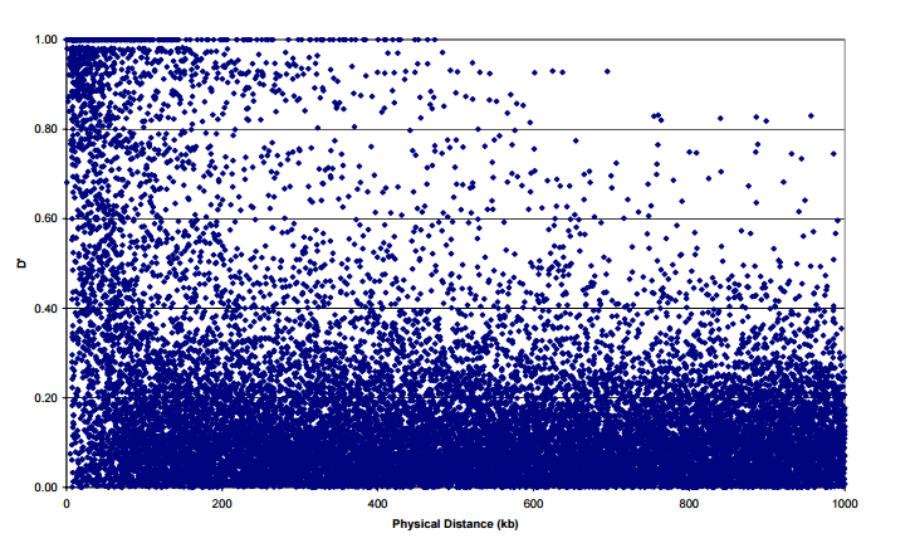
\includegraphics[scale=0.25]{d22}
				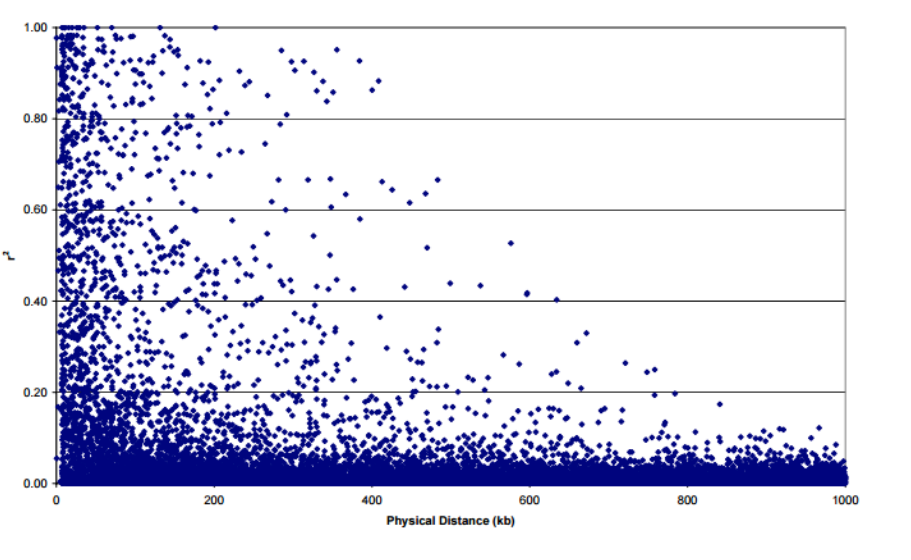
\includegraphics[scale=0.25]{r22}
				\caption{Top: raw data for D' from chr22.\\
				Bottom: raw data for $r^2$ from chr22. The trend is the same, but being the measure less strong we see a decrease in density of high values.
				}
				\label{fig:compare}
				\end{figure}
				
			\subparagraph{Detailed visualization of LD}
			A useful visualization of the LD, which will come in handy when dealing with haplotypes, is the representation through a matrix. 
			In this example (figure \ref{fig:visual}), we have 6 SNPs for which we are calculating the LD repeated both on the y and x axis, ordered by genomic coordinates. 
			The two parts of the matrix divided by the diagonal are used to visualize the $D'$ and $r^2$ relation across all pairs of SNPs.
			
			\begin{figure}[H]
				\centering
				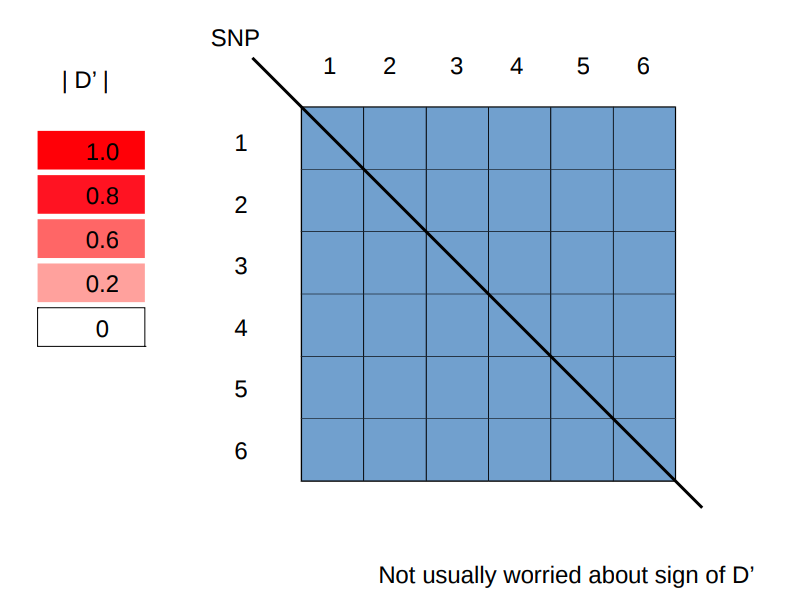
\includegraphics[scale=0.2]{vis1}
				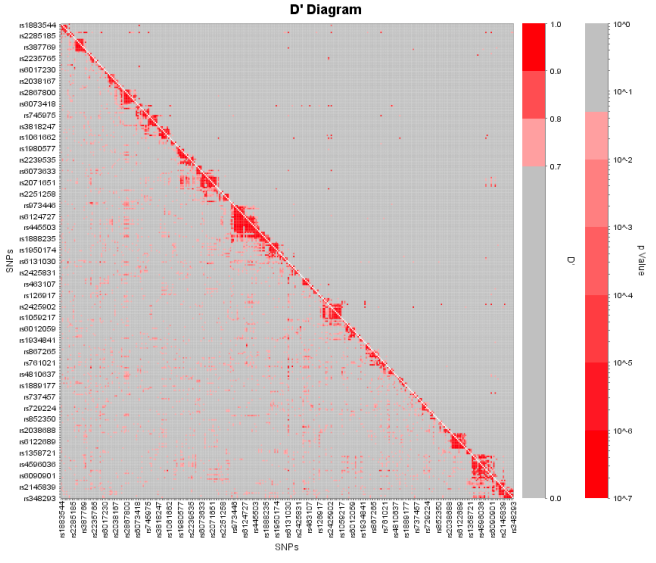
\includegraphics[scale=0.3]{vis2}
				\caption{Top: Schematic representation of the matrix\\
				Bottom: real example. we can see block that cluster together. Triangles arising on the diagonal are SNPs strongly correlated, not casual pattern in the population. These are \textbf{haplotype blocks}. }
				\label{fig:visual}
				\end{figure}
			

			\paragraph{Haplotypes}
			An haplotype is a set of linked SNPs on the same chromosome.
			
			\begin{figure}[H]
				\centering
				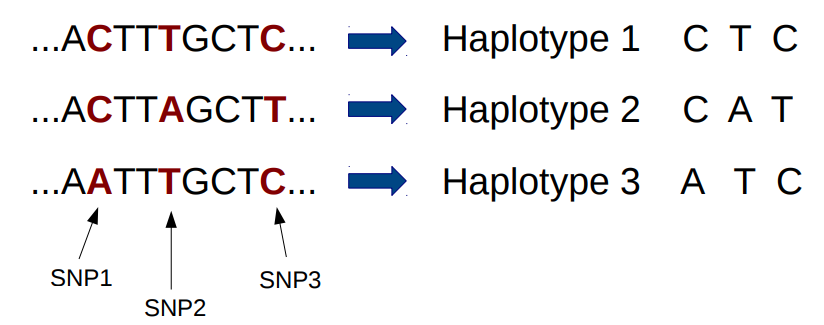
\includegraphics[scale=0.3]{haplo}
				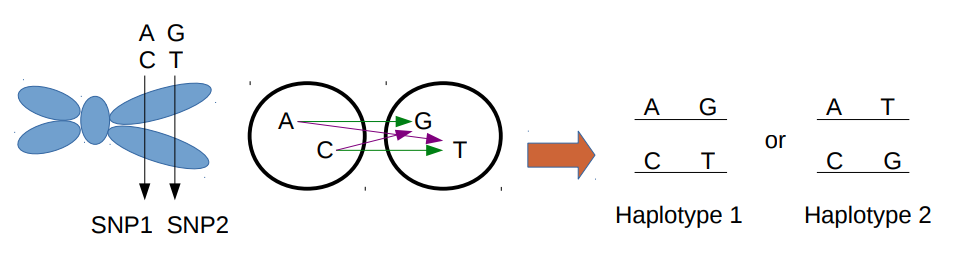
\includegraphics[scale=0.3]{haplo2}
				\caption{Remember that when when talking about haplotypes we also need first to somehow reconstruct and assign a so called "phased" genotype so we know how the SNPs are disposed in the two alleles. Only after having a clear view of the genotype we can reason in terms of haplotype, comparing the genetic profiles  }
				\label{fig:haplo}
				\end{figure}
				
			Genotypes don't report information about the connections of alleles at different SNPs loci, so there could be several possible haplotypes for the same genotype (bottom figure in \ref{fig:haplo}).
			An haplotype block is defined as a cluster of SNPs in linkage disequilibrium and an haplotype boundary as sequences of blocks with strong internal linkage disequilibrium but no linkage disequilibrium between them.
			They usually reflect genetic recombination hotspots.

			\paragraph{Tag SNPs}
			Tag SNPs are a set of SNPs that captures most variations in haplotypes, removing redundancy.
			If the linkage is extremely strong it is enough to have one (tag) SNP to retrieve the information about other SNPs.
			Tag SNPs allow for computationally feasible GWAS.
			\\
			There are different platforms to identify SNPs, one of the main used being GeneChip Human Mapping microarray, provided by Affymetrix. 

		\subsubsection{SNP genotyping}
		In microarray technologies, SNP genotyping represents each SNP in the dimension of its $A$ and $B$ allele intensity.
		The genotype of an individual (monozygous for $A$, monozygous for $B$, heterozygous) is retrieved by comparing the intensity of the fluorescent signal (figure \ref{fig:geno}). 
		
		\begin{figure}[H]
				\centering
				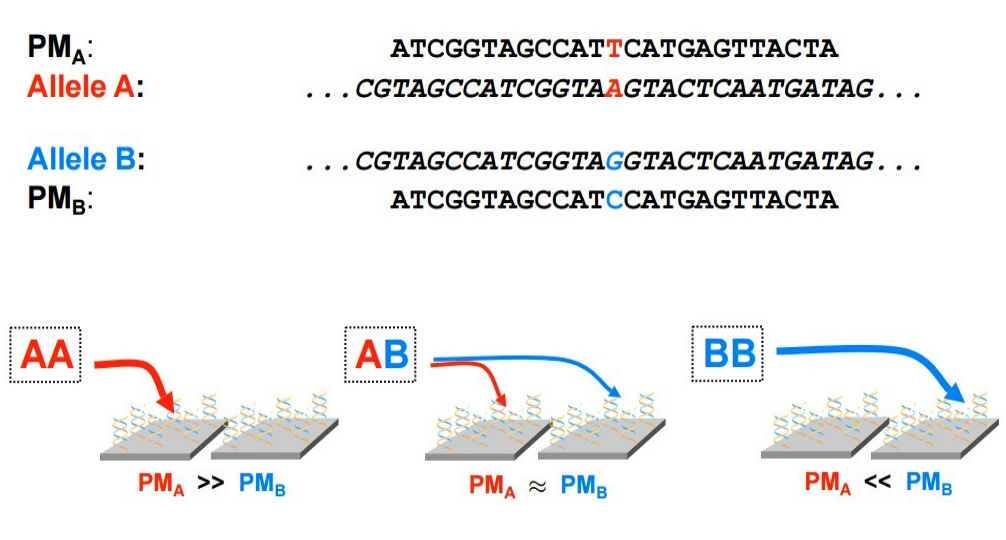
\includegraphics[scale=0.3]{genotype}
				\caption{SNPs genotyping in microarray technologies. For individuals having genotype, for example, $AA$, we expect to have much more signal in probes carrying the $A$ }
				\label{fig:geno}
				\end{figure}
				
			Not all SNPs have a clear representation, however, in the classical two-dimensional visualization.
			For this reason, other methods to analyze the output images of the machine have been developed, like \textbf{Birdseed} by Affymetrix, or CRLMM.

			\paragraph{Birdseed}
			A method to call the genotype is Birdseed\footnote{This paragraph draws an interesting bridge between the expression arrays (RNA), seen in chapter 5, with genotyping arrays (DNA)}.
			Given a set of data coming from different individuals, tries to infer their genotype based on how these intensities are disposed on the bi-dimensional space of the image.
			A canonical, satisfying result is similar to the one in figure \ref{fig:birdseed}. 
			Each point represents an individual. 
						
			
			\begin{figure}[H]
				\centering
				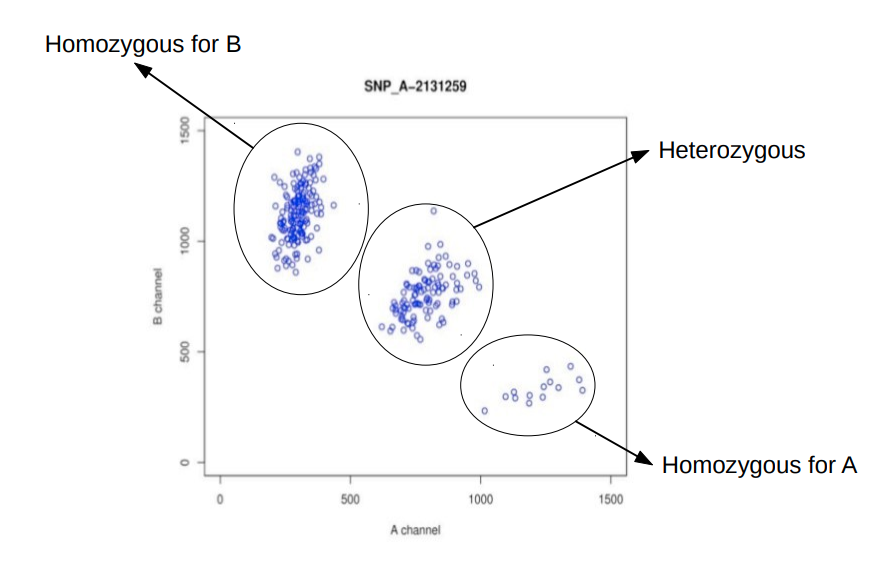
\includegraphics[scale=0.3]{birdseed}
				\caption{Classical good result of Birdseed. }
				\label{fig:birdseed}
				\end{figure}
			
			
			Birdseed is a \textbf{clustering algorithm} that first construct training models for each SNP in the array and then compute SNPs genotyping on data of interest using the training models.
			The high-level functioning can be summarized in two main steps:
			\begin{enumerate}
			\item Construct "training" models for each SNP in the array (data with known genotype);
			\item Compute SNPs genotyping on data of interest using the training models. 
			\end{enumerate}
			
			Each SNP is a bird\footnote{Because if the three clusters are connected, it looks like a bird, apparently.}, where its wing points are genotypes $AA$ and $BB$ and the body is $AB$.
			Birds are computed for all SNPs.
			Then Birdseed estimates cluster centers and covariance matrices.
			Its confidence is computed as:

			$$Confidence = 80\% E_1 + 20\% E_2$$

			Where $E_1$ is the posterior to the second closest peak over the posterior to the closest and $E_2$ is the deviation penalty from the closest peak.
			Then the quality score is computed as:

			$$QS = -\log_{10}(confidence + 0.00001)\cdot 2000$$
			
			\begin{figure}[H]
				\centering
				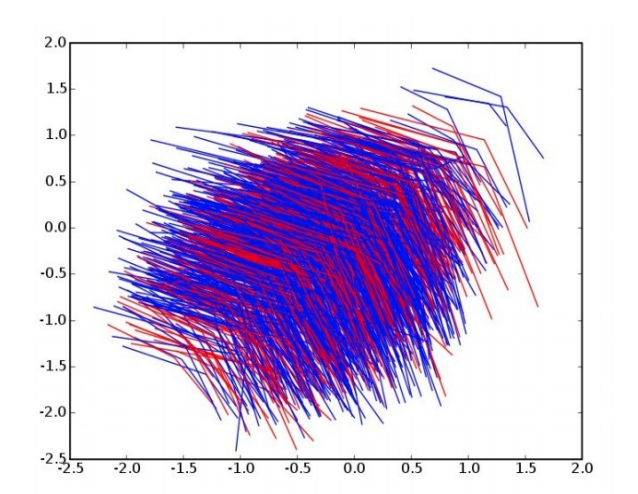
\includegraphics[scale=0.3]{bird1}
				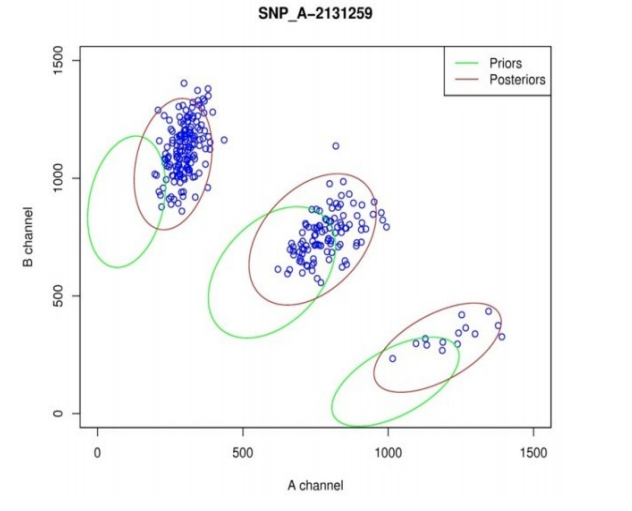
\includegraphics[scale=0.3]{bird2}
				\caption{Birdseed can make highly accurate predictions because it has learned cluster morphology patterns by studying flocks of birds.\\
				Birdseed uses a highly customized EM algorithm using the SNP-specific bird as the "seed" (hence the name) and as cluster anchors. For each SNP in a dataset we can know the quality of the genotyping, given some \textit{a priori} information. }
				\label{fig:birdseed1}
				\end{figure}
			

			\paragraph{SNP genotyping from NGS data}
			While microarray technologies are still sometimes used, since they give decent, precise results, nowadays they are being replaced by NGS sequences. 
			However, microarrays are still particularly relevant in GWAS, since these analyses are carried for thousands of individuals and microarrays are way cheaper. 
			The real potential of NGS for SNPs genotyping lies in the fact that NGS can capture all SNPs, even rare ones that are not captured by array technologies, which focus on common SNPs. 			\\
			To genotype SNP from NGS the \textbf{pileup} is used.
			After the reads are aligned and the \textbf{coverage} computed, the pileup is the count of the number of times the reference and the alternative reads appear.
			From this the \textbf{allelic fraction} can be computed.
			\\
			The main tools for SNP calling in NGS data are Samtools, Bcftools, Vcftools, GATK.

			\paragraph{Quality control}
			Quality control is essential, since low-quality reads can introduce bias and produce unwanted artifacts.
			To perform quality control of SNP genotyping:

			\begin{multicols}{2}
				\begin{itemize}
					\item Subjects with missing call rate less than $1$ or $5\%$ are filtered out because of poor DNA quality.
					\item SNP with genotype call rates less than $5\%$ are filtered out because of errors, noise and non-specific probes.
					\item SNPs with minor allele frequencies less than $1\%$ are filtered out because they are error prone and unpowered.
					\item SNPs are filtered out by testing for HW equilibrium: a deviation can indicate genotyping errors, batch effects or a change in the genetic structure.
				\end{itemize}
			\end{multicols}

		\subsubsection{Independence of individuals}
		Independence among samples is a fundamental assumption of case-control studies, so related individuals are excluded, or their association taken into account during association analysis.
		Genomic distance between samples can be computed based on SNP profiles through genetic fingerprinting or through \textbf{SPIA}:

		$$D(CL_1, CL_2) = \frac{1}{vN_{SNPs}} \sum\limits_{i=1}^{N_{SNPs}} \neg\delta(CL_{1i}, CL_{2i})$$

		\subsubsection{Genetic structure}
		Not everyone in the population has the same genetic background: some people are more genetically similar than others.
		Admixed population are particularly interesting and many SNPs in the genome have different distribution between different population due to random drift.
		Many traits have strong population association, so the genetic background of individuals of a cohort must be taken into account to avoid structure and stratification of the samples.
		
		Traits having strong population association are, for example, diabetes, which in the US in much more common among blacks; or Crohn's disease, wirh in Israel is more common among Ashkenazi Jews.
		When designing a case control study, if population stratification is not the same in case and control sets, we may find signals that are not related to the disease, but just related to the difference in proportions of population.
		
		The degree of admixture and population of origin identification is important.
		This can be done through SNP-based or model-based methods.

			\paragraph{Logistic regression}
			Logistic regression is a variation of regression analysis, developed to deal with binary phenotypes.
			It is a method used to assess the associations of SNPs and outcomes.
			The better the fit the stronger the association.
			It is computed as:

			$$\log(\frac{\pi}{1-\pi}) = \beta_0+\beta_1x_1+\cdots \beta_mx_m$$

			Where $x_i$ are the SNP genotype and $\beta$ the covariates like age, sex and population structure.
			Then genetic structure correction is performed through $QQ$ plots (figure \ref{fig:qq}), where deviation from the diagonal indicates structure.
			The data is fitted to the diagonal as to reduce structures effects.

			
			\begin{figure}[H]
			\centering
			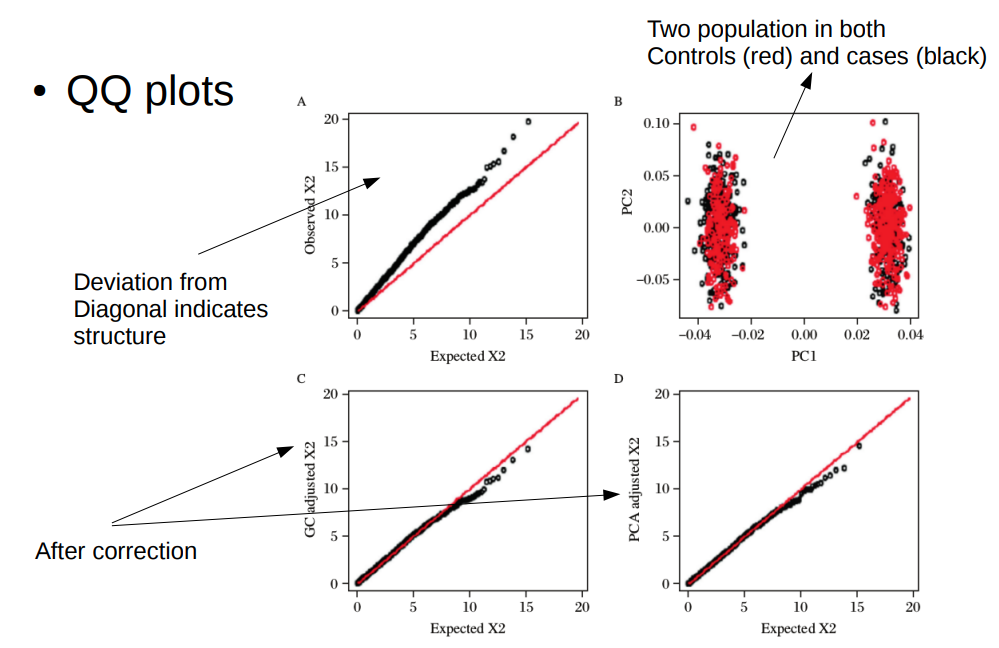
\includegraphics[scale=0.3]{qq}
			\caption{First row: unexpected deviation, probably given by population stratification. We can calculated the two principal components of the case-control, and add to our logistic regression model these two eigenvectors to correct for the supposed stratification. After the correction we can see that the obtained p-value distribution is much closer to the expected one. Indeed in a normal scenario we expect most of the SNPs not to be associated, with only a tail of p-values diverging from the distribution only in case of a real signal. In this case we can say that our GWAS analysis is trustful. }
			\label{fig:qq}
			\end{figure}
	
	\subsection{Standard cutoff in GWAS}
	We need a measure for the significance of association.
	Considering evidence for $1M$ haplotype blocks in the genome, the accepted p-value cutoff in GWAS studies is between $10^{-6}$ and $10^{-8}$.
	This is due to the fact that each SNP is tested at the traditional significance level and multiple comparison is an important consideration in a GWAS analysis and must be handled properly.

	\subsection{Independent replication}
	Independent replication is used to evaluate systemically whether or not the discovered SNPs in initial GWAS are spurious signals.
	Samples are collected the same way as the original study and the association is computed with the same genetic model.
	The effect sizes of marker should show the same signs in both the replicated and original study.
